\cotefile{79}
\scanpage{33}
\figure{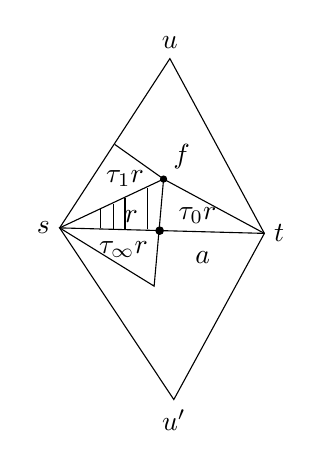
\begin{tikzpicture}[x=1cm,y=1cm,baseline]
\coordinate (s) at (0,0); \coordinate (t) at (2.6,-.07);
\coordinate (u) at (1.4,2.15); \coordinate (v) at (1.45,-2.18);
\coordinate (f) at (1.32,.62); \coordinate (a) at (1.27,-.035);
\draw (s)--(u)--(t)--(v)--cycle (s)--(t);
\draw (.70,1.06)--(f)--(t) (s)--(f)--(1.20,-.74)--cycle;
\foreach \x in {.52,.68,.83,1.12}{\draw (\x,-.013*\x)--(\x,.45*\x);}
\fill (f) circle (.046) (a) circle (.055);
\node[left] at (s){$s$}; \node[right] at (t){$t$};
\node[above] at (u){$u$}; \node[below] at (v){$u'$};
\node[above right] at (f){$f$}; \node[below right] at (1.60,-.18){$a$};
\node at (.83,.63){$\tau_1 r$}; \node at (1.75,.16){$\tau_0 r$};
\node at (.81,-.27){$\tau_\infty r$}; \node at (.91,.15){$r$};
\end{tikzpicture}}

Si $u'$ est le sommet de $SP_M$ tel que l'on ait
\[
\{s,t,u'\}\in SF_M \qquad \{s,t,u'\}\ne\{s,t,u\}\quad\text{i.e. }u'\ne u
\]
i.e.
\[
u'=(x-y)^{\bullet},\tag*{(81)}
\]
on aura
\[
\left\{\begin{aligned}
\tau_0^r(s,t,u)&=(t,s,u)\\
\tau_1^r(s,\deleted{\unsure{b}}t,u)&=(s,u,t)\\
\tau_\infty^r(s,t,u)&=(s,t,u')
\end{aligned}\right.
\qquad\text{\deleted{\illegible{1} est le \unsure{sommet}}}\tag*{(81)}
\]
donc $\tau_0^r,\tau_1^r,\tau_\infty^r$ sont induits respectivement par les automorphismes \inserted{antisymplectiques} de $M$, \unsure{qui|que} \deleted{\unsure{transf}}\deleted{\unsure{transforment}} sont caractérisés par
\[
\left\{\begin{aligned}
\tau_0^r\;&\left\{\begin{aligned}x&\mapsto y\\y&\unsure{\vdash\!\dashv|\mapsto}x\\z&\mapsto z\end{aligned}\right.
&&\text{matrice }\begin{pmatrix}0&1\\1&0\end{pmatrix}=r_0^{\deleted{\unsure{r}}}\\[3pt]
\tau_1^r\;&\left\{\begin{aligned}x&\mapsto x\\y&\mapsto \deleted{\unsure{y}}z\\z&\unsure{\vdash|\mapsto}y\end{aligned}\right.
&&\text{matrice }\begin{pmatrix}1&-1\\0&-1\end{pmatrix}=-r_1\\[3pt]
\tau_\infty^r\;&\left\{\begin{aligned}x&\mapsto x\\y&\mapsto-y\\z&\mapsto y-x\end{aligned}\right.
&&\text{matrice }\begin{pmatrix}1&0\\0&-1\end{pmatrix}=-r_\infty
\end{aligned}\right.\tag*{(82)}
\]
les automorphismes correspondants de $M$, et leurs matrices p.r. à la base $(x,y)$ de $M$, sont déterminés modulo signe par le choix du repère $r$ (et $=$, pour ce qui est des matrices, indépendamment du choix du repère). On trouve
\[
\left\{\begin{aligned}
\rho_0^r&\overset{\mathrm{déf}}{=}\tau_\infty^r\tau_1^r\mapsto\begin{pmatrix}1&-1\\0&1\end{pmatrix}=\lambda_0\\
\rho_1^r&\overset{\mathrm{déf}}{=}\tau_0^r\tau_\infty^r\mapsto\begin{pmatrix}0&-1\\1&0\end{pmatrix}=-\lambda_1\\
\rho_\infty^r&\overset{\mathrm{déf}}{=}\tau_1^r\tau_0^r\mapsto\begin{pmatrix}-1&1\\-1&0\end{pmatrix}=-\lambda_\infty
\end{aligned}\right.,\tag*{(83)}
\]
i.e. à des différences de signe près (qui du reste
% archive sheet number: 32
